\documentclass[12pt, a4paper]{article}
\usepackage{geometry}
\geometry{margin=2.5cm}
\usepackage{graphicx}
\usepackage{amsmath}
\usepackage{enumitem}
\usepackage[utf8]{inputenc}
\usepackage[french]{babel}
\usepackage{listings}
\usepackage{xcolor}
\title{SAÉ 3.01 Rapport de cryptographie}
\author{Jules CHIRON, Matis RODIER, Thomas GODINEAU | INF2 FI A}
\date{4 janvier 2024}

\usepackage[T1]{fontenc}
\begin{document}
\maketitle

\begin{figure}[h]
    
\includegraphics[width=0.6\textwidth]{../annexes/logo_uvsq}
\end{figure}

\tableofcontents{}
\section*{Introduction}
\addcontentsline{toc}{section}{Introduction}

Le but de cette SAÉ est de réaliser une \textbf{application web} de ticketing en PHP.\@
Chaque utilisateur de cette plateforme peut créer un compte et se connecter.
Afin de sécuriser les mots de passe des utilisateurs, nous les chiffrons avec l'algorithme \textbf{RC4}.
\bigskip

La \textbf{première partie} de ce rapport contient le code PHP commenté des modules de chiffrement et de déchiffrement.
La \textbf{deuxième partie} contient une recherche documentaire sur les fonctions de hachage cryptographique,
l'algorithme MD5 et les applications de ces algorithmes en cryptographie.

\section{Algorithme RC4}

\subsection*{Permutation et suite chiffrante}

Pour ce module,
nous avons utilisés les algorithmes écrit en pseudo-code fournis dans le sujet.
Il y a juste un changement dans la fonction \textit{gen} (ligne 11).

\lstset{
    language        = php,
    backgroundcolor = \color{gray!3},
    inputencoding   = utf8,
    title           = \lstname,
    literate        = {è}{{\`e}}1 {é}{{\'e}}1 {à}{{\`a}}1 {î}{{\^\i}}1,
    frame           = single,
    basicstyle      = \small\ttfamily,
    keywordstyle    = \color{blue!80!black},
    stringstyle     = \color{red},
    identifierstyle = \color{green!40!gray},
    commentstyle    = \color{orange},
    emph            = [1]{php},
    emphstyle       = [1]\color{black},
    emph            = [2]{if,and,or,else},
    emphstyle       = [2]\color{yellow!80!black},
    numbers         = left,
}

\begin{lstlisting}[name=Fonction de génération de la permutation]
function ksa($k){
    // On crée un tableau de caractères à partir de la clé
    $k = str_split($k);
    
    for ($i = 0; $i < count($k); $i++){
        // On récupère le code ASCII de chaque caractère
        $k[$i] = intval(ord($k[$i]));
    }

    $s = array();
    for ($i = 0; $i < 256; $i++){
        // On crée un tableau de 0 à 255
        $s[] = $i;
    }

    $j = 0;
    for ($i = 0; $i < 256; $i++){
        // On mélange le tableau de manière à obtenir
        // une permutation des 256 valeurs
        $j = ($j + $s[$i] + $k[$i % count($k)]) % 256;
        $temp = $s[$i];
        $s[$i] = $s[$j];
        $s[$j] = $temp;
    }

    return $s;
}
\end{lstlisting}

\begin{lstlisting}[name=Fonction de génération de la suite chiffrante]
function gen($s, $n){
    $j = 0;
    $k = array();

    for ($i = 0; $i < $n; $i++){
        // On initialise le tableau de sortie avec n 0
        $k[] = 0;
    }
    
    $i = 0;
    for ($l = 0; $l < $n; $l++){ // /!\ Changement dans le sujet
        $i = ($i + 1) % 256;
        // On récupère la valeur du tableau à l'indice i
        // et on l'ajoute à j
        $j = ($j + $s[$i]) % 256;

        // On échange les valeurs de s[i] et s[j]
        $temp = $s[$i];
        $s[$i] = $s[$j];
        $s[$j] = $temp;

        // On modifie la valeur de k à l'indice l
        // avec la valeur de s à l'indice (s[i] + s[j]) % 256
        $k[$l] = $s[($s[$i] + $s[$j]) % 256];
    }

    return $k;
}
\end{lstlisting}

\subsection*{Chiffrement et déchiffrement}

\begin{lstlisting}[name=Fonction de chiffrement]
function cypher($m, $k){
    $m = str_split($m);
    
    // On génère la suite chiffrante
    $s = gen(ksa($k), 128);

    for ($i = 0; $i < count($m); $i++){
        // On récupère le code ASCII de chaque caractère du message
        $m[$i] = intval(ord($m[$i]));
    }

    $c = array();
    for ($i = 0; $i < count($m); $i++){
        // On effectue un XOR entre le message et la suite

        // On convertit le résultat en hexadécimal
        // et on l'ajoute au tableau de sortie
        if (strlen(dechex($m[$i] ^ $s[$i])) == 2)
            $c[] = dechex($m[$i] ^ $s[$i]);
        else
            // Si le code ASCII est inférieur à 16,
            // on ajoute un 0 devant le résultat
            $c[] = '0'.dechex($m[$i] ^ $s[$i]);
    }

    // On retourne le résultat sous forme de chaîne de caractères
    return implode('', $c);
}
\end{lstlisting}

\begin{lstlisting}[name=Fonction de déchiffrement]
function decypher($c, $k){
    $c = str_split($c, 2);
    $s = gen(ksa($k), 128);

    for ($i = 0; $i < count($c); $i++){
        // On convertit chaque caractère hexadécimal en décimal
        $c[$i] = hexdec($c[$i]);
    }

    $m = array();
    for ($i = 0; $i < count($c); $i++){
        // On effectue un XOR entre le message chiffré et la suite
        $m[] = chr($c[$i] ^ $s[$i]);
    }

    return implode('', $m);
}
\end{lstlisting}

\section{Travail de recherche}

\subsection{Fonction de hachage cryptographique}

\subsection*{Définition}
Une fonction de hachage cryptographique est une fonction qui associe à un message d'entrée
(chaîne de caractères, entier …) une valeur bien précise appelée “empreinte”.

\subsection*{Propriétés}\label{hash_properties}

Une fonction de hachage doit disposer de certaines propriétés afin d'être suffisamment sûre et efficace.
Premièrement, la taille des empreintes doit être \textbf{indépendante de la longueur} du message.
Deuxièmement, une fonction de hachage doit renvoyer \textbf{une seule et unique empreinte} pour chaque message possible.

À l'inverse, elle doit renvoyer \textbf{deux empreintes différentes} pour deux messages différents.
Si ce n'est pas le cas, il y a alors des \textbf{collisions} et l'algorithme n'est plus sûr
car deux messages différents peuvent être utilisés alors qu'un seule est le bon (s'ils ont la même empreinte).
Si ces messages ne diffèrent même que très peu, les empreintes des deux messages doivent être \textbf{très différentes}
 afin de ne pas pouvoir s'approcher de plus en plus du message en essayant de décrypter une empreinte.
Enfin, il ne doit \textbf{pas être possible de retrouver un message} à partir de son empreinte (du moins sans la clé).

\subsection{Chiffrement MD5}

\subsubsection*{Présentation}\label{md5_presentation}

La \textbf{fonction de hachage MD5} est une fonction de hachage cryptographique.
MD5 est l'acronyme de Message Digest 5 (équivalent d'\textit{empreinte} en français et \textit{5} car il succède au \textbf{MD4}).
Cette fonction a été inventée par \textbf{Ronald Rivest} (un des inventeurs du \textit{RSA}) en 1991,
c'est l'amélioration de l'algorithme \textbf{MD4}.
Cependant, de graves failles de sécurité ont été découvertes en 1996,
et des collisions ont été trouvées en 2004 par une équipe chinoise.
Ainsi, l'\textbf{algorithme MD5} n'est plus considéré comme sûr et est déconseillé pour des applications cryptographiques.
D'autres algorithmes plus récents et plus sûrs ont été créés et sont recommandés pour des applications dans ce domaine,
comme \textbf{SHA-256}.
Cependant, MD5 est encore utilisé pour vérifier l'intégrité de fichiers (pour vérifier qu'ils n'ont pas été modifiés)
lors de téléchargements.

\subsection*{Fonctionnement}

L'empreinte de l'\textbf{algorithme MD5} est une chaîne de 128 bits (16 octets donc 16 caractères).
La \textbf{fonction MD5} travaille sur des blocs de 512 bits (soit 64 caractères).
Si la longueur du dernier bloc du message n'est pas un multiple de 448 bits, il est complété:
\begin{itemize}
    \item On ajoute un 1 à la fin du message
    \item On ajoute des 0 jusqu'à ce que la longueur du dernier bloc soit égale à 448 bits
\end{itemize}
\bigskip
On ajoute ensuite la taille du message (\textbf{sur 64 bits}) à la fin de celui-ci.
La longueur du message est donc maintenant un multiple de 512 bits ($448 + 64 = 512$).
Le message est donc ensuite découpé en bloc de 512 bits.

Suite à cela, on calcule 64 constantes de 32 bits (\textit{64 mots}) que l'on stocke dans un tableau à partir de la fonction sinus:
\[
    \forall i \in [1, 64],\
    K[i] = \lfloor 2^{32} \times \left | \sin(i) \right | \rfloor
\]
On définit également un tableau de 64 cases contenant des valeurs qui seront utilisées pour effectuer des rotations de bits:
\[
    S = \left [
        [7, 12, 17, 22] \times 4, [5, 9, 14, 20] \times 4, [4, 11, 16, 23] \times 4, [6, 10, 15, 21] \times 4 \right ]
\]
On choisit 4 valeurs arbitraires de 32 bits (L, M, N et O) et on définit les 4 fonctions suivantes:
\begin{itemize}
    \item $F(X, Y, Z) = (X \wedge Y) \vee (\bar X \wedge Z)$
    \item $G(X, Y, Z) = (X \wedge Z) \vee (Y \wedge \bar Z)$
    \item $H(X, Y, Z) = X \oplus Y \oplus Z$
    \item $I(X, Y, Z) = Y \oplus (X \vee \bar Z)$
\end{itemize}
\bigskip
En francais cela donne:
\begin{itemize}
    \item $F(X, Y, Z) = (X \ ET \ Y) \ OU \ (NON \ X \ ET \ Z)$
    \item $G(X, Y, Z) = (X \ ET \ Z) \ OU \ (Y \ ET \ NON \ Z)$
    \item $H(X, Y, Z) = X \ XOR \ Y \ XOR \ Z$
    \item $I(X, Y, Z) = Y \ XOR \ (X \ OU \ NON \ Z)$
\end{itemize}
\bigskip
Puis, \textbf{chaque bloc} est traité de la manière suivante:
\begin{itemize}
    \item On initialise 4 variables de 32 bits (A, B, C et D) avec les valeurs initiales
    \item On effectue 64 tours de boucle (on effectue $4 \times 16$ opérations) avec les fonctions $F$, $G$, $H$ et $I$
    (fonctions $F$ pour les 16 premières, puis $G$ pour les 16 suivantes \ldots) (voir Figure~\ref{md5_algo}):
    \begin{itemize}[label={\textbullet}]
        \item On applique la fonction (\textit{F, G, H ou I}) aux variables B, C et D
        \item On ajoute le résultat de la fonction à la variable A
        \item On ajoute aussi à A la valeur du message à l'indice \textit{i} (le tour de boucle) et $K[i]$
        \item On effecture une rotation de A de $S[i]$ bits vers la gauche
        \item On ajoute B à A
        \item On applique modulo $2^{32}$ à A
        \item Enfin, On effectue une rotation des variables A, B, C et D ($A \rightarrow B, \ B \rightarrow C, \ C \rightarrow D, \ D \rightarrow A$)
    \end{itemize}
    \item On ajoute les valeurs des variables A, B, C et D aux valeurs initiales ($L = L + A$, $M = M + B$, \ldots)
    \item On recommence pour chaque bloc
\end{itemize}
\bigskip
Enfin, on concatène L, M, N et O pour obtenir \textbf{l'empreinte finale du message} ($4 \times 32 = 128 \ bits$).
\bigskip
\begin{figure}[ht]
    \centering
    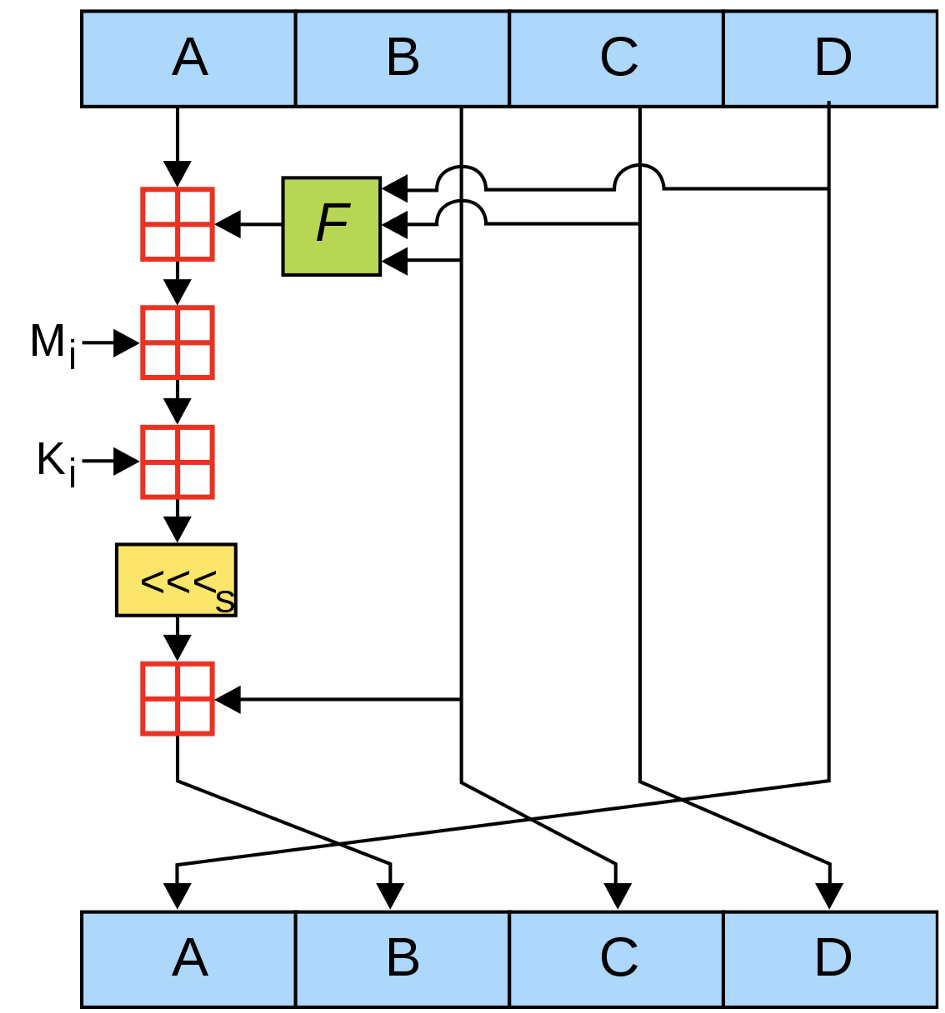
\includegraphics[width=0.4\textwidth]{../annexes/md5_algo.png}
    \caption{Représentation d'une des 64 itérations de l'algorithme MD5}\label{md5_algo}
\end{figure}

\subsection{Utilisation dans la cryptographie}

Les \textbf{fonctions de hachage} telles que \textbf{MD5} trouvent un intérêt dans la cryptographie.
Effectivement, ces fonctions transforme un \textbf{message} (chaîne de caractères, entier \ldots) en une \textbf{empreinte}
(chaîne de caractères représentant une suite hexadécimale) dont la taille ne dépend pas de la taille du message.

\noindent De plus, on peut observer que si on modifie un caractère du message, l'empreinte finale change complètement.
On ne peut donc pas déchiffrer un message à partir de son empreinte (\textit{à tatillon}).

\noindent Enfin, (\textit{pour l'algorithme MD5}) il existe théoriquement \textbf{plus de $\mathbf{3\times 10^{38}}$}
empreintes différentes pouvant être possiblement générées
($2^{128} = 3,402823669 \times 10^{38}$).
Il est donc très peu probable de trouver deux messages différents ayant la même empreinte
(\textit{outre les collisions découvertes en 2004 (cf~\ref{md5_presentation})}).

\bigskip
Ainsi, des fonctions telles que \textbf{MD5} ou encore \textbf{SHA-256} vérifient les différentes propriétés
que nous avons énoncées dans la partie~\ref{hash_properties}. C'est pourquoi de telles fonctions sont utilisées
dans la cryptographie.

\end{document}
